\doublespacing % Do not change - required

\chapter{Literature Review}
\label{ch2}

%%%%%%%%%%%%%%%%%%%%%%%%%%%%%%%%%%%%%%%
% IMPORTANT
\begin{spacing}{1} %THESE FOUR
\minitoc % LINES MUST APPEAR IN
\end{spacing} % EVERY
\thesisspacing % CHAPTER
% COPY THEM IN ANY NEW CHAPTER
%%%%%%%%%%%%%%%%%%%%%%%%%%%%%%%%%%%%%%%


\section{Historical Development of Energy Monitoring Systems}

The development of energy monitoring systems began with the increasing need for energy efficiency and consumption management. While only manual meter readings and periodic energy audits were performed at first, an evolution towards more continuous and real-time monitoring took place over time. Especially after the energy crisis in the 1970s, feedback systems began to be developed in order to change consumers' energy usage habits and increase efficiency.

In the early 2000s, the integration of SCADA and PLC-based systems into the field of industrial energy monitoring gained momentum. SCADA systems have become an important step in energy management by offering data collection, visualization and remote control functions together. PLCs, on the other hand, have contributed to automation processes with their high reliability and fast processing capacities.

On the building and residential scale, the use of smart meters has started a new era. Thanks to smart meters, not only total consumption but also consumption data separated by different time periods and devices can be collected. This development has played a critical role in increasing consumer awareness and supporting demand-side management applications.
In the 2010s, IoT (Internet of Things)-based solutions have become widespread in energy monitoring systems. It has become possible to collect, analyze and visualize instant data using IoT devices, sensors and cloud-based data processing platforms. Low-cost and powerful devices, such as Raspberry Pi, have begun to be used extensively in real-time energy monitoring projects in industrial facilities and buildings. In addition, it has become important not only to measure energy consumption but also to quickly detect critical changes with event-based monitoring. Instead of traditional time-based data collection methods, methods based on recording data when there is a significant change in energy use have been developed. Today, energy management systems supported by AI (Artificial Intelligence) and Big Data analytics are developing. These systems can analyze large volumes of data to detect anomalies, make consumption estimates and develop automatic optimization strategies.

\section{Modbus Based Energy Monitoring}

Modbus-based energy monitoring systems are widely used in industrial and commercial facilities that provide real-time and precise monitoring of electrical parameters (such as current, voltage, power, energy consumption). Modbus is preferred as the basic communication protocol in these systems. Developed in 1979, the Modbus protocol has become indispensable in energy monitoring systems thanks to its open standard structure, low-cost ease of implementation, and wide device compatibility.
Modbus collects data from energy analyzers, meters, and various monitoring devices and transfers data to a central server or software. This structure allows the system to operate reliably even in large-scale field applications.
Energy monitoring systems generally consist of measuring devices such as energy analyzers or smart meters, an RS-485 communication line, a data collection server, and user-friendly monitoring software. Data is collected using Modbus RTU or TCP/IP protocols and then recorded in databases and visualized in graphical interfaces.
For example, in the study titled "Development of a Real-Time Energy Monitoring Platform User-Friendly for Buildings", energy consumption data was transferred to the Arduino Mega 2560 microcontroller via the RS485 line with the Modbus RTU protocol. The collected data was transmitted to the server via the Ethernet module and visualized in real time in the web-based interface developed using the Node-RED platform.
\begin{figure}[H]
    \centering
    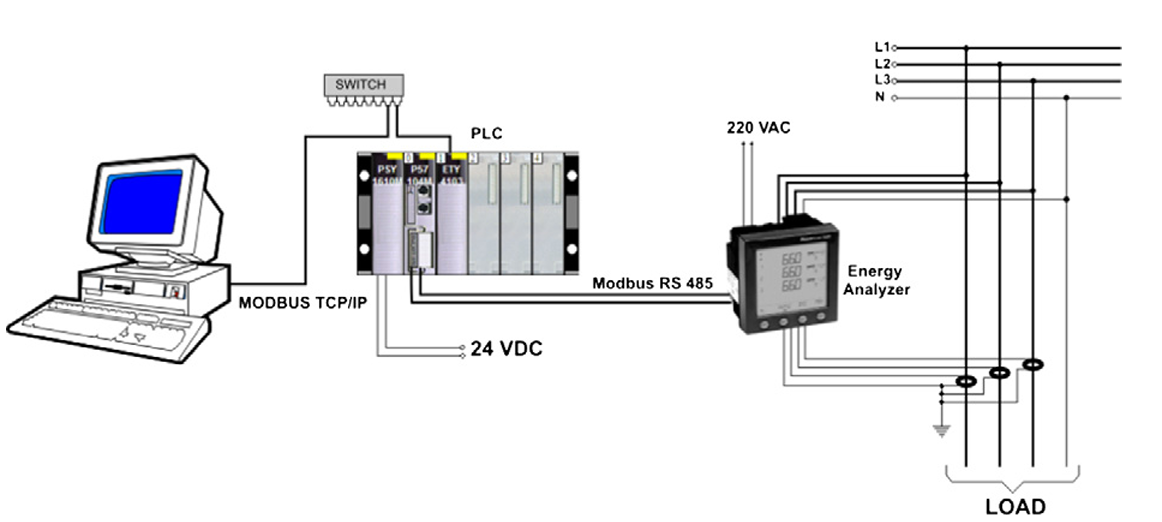
\includegraphics[width=0.8\columnwidth]{imgs/Schema of the proposed energy monitoring system.png}
    \caption[Short description for list of figures]{Schema of the proposed energy monitoring system }
    \label{fig-magnitude}
    \end{figure}%

    The reasons why Modbus-based energy monitoring systems are preferred are their open standard structure, easy expansion of the systems, compatibility with devices from different manufacturers, and low processing power requirements. Thanks to these systems, instant energy consumption in facilities can be monitored, measures can be taken to reduce consumption during peak load times, and overall energy efficiency can be increased. In addition, recording real-time consumption data allows for more accurate billing and the development of energy saving strategies by analyzing consumption habits.
    
    Advantages and disadvantages of Modbus communication protocol:
    \begin{table}[htbp]
        \centering
        \caption{Advantages and Disadvantages of Modbus Protocol}
        \begin{tabular}{|p{7cm}|p{7cm}|}
        \hline
        \textbf{Advantages} & \textbf{Disadvantages} \\
        \hline
        Open Standard: The Modbus protocol is free to use and compatible with devices from different manufacturers. &
        Limited data security: The Modbus protocol does not inherently have encryption or authentication mechanisms; extra security measures must be taken. \\
        \hline
        Easy integration: Many measuring devices can be easily connected to the network via RS-485 or TCP/IP infrastructure. &
        Slow data rate: Physical layers such as RS-485 offer low bandwidth, performance may be limited where very heavy data flow is required. \\
        \hline
        Low cost: Hardware and implementation costs are lower than other protocols. &
        Master-slave dependency: Due to the Modbus structure, only the master device initiates the query; the slave cannot send data on its own. \\
        \hline
        Wide industrial application: It has become the standard in many sectors such as power plants, factories, shopping malls, data centers. &
        Address limitation: Classic Modbus RTU networks have a theoretical limit of 247 devices. Larger networks require additional solutions. \\
        \hline
        \end{tabular}
        \label{tab:modbus_comparison}
        \end{table}
        



\section{Recommended Approaches}

As a real application, in the study titled "Automatic Meter Reading with LabVIEW Program for Real-Time Energy Monitoring and Consumer Awareness", a highly effective method has been developed in terms of energy saving and grid load balance. In the study, firstly, energy consumption data was collected instantly from smart meters installed in the field using RS-485 communication protocol. This data was processed with NI LabVIEW™ software and presented to consumers in a user interface both numerically and graphically. Thus, users were able to see their daily and instant energy consumption in detail and analyze their own consumption habits without waiting for billing periods. Not only monitoring software was used in the system infrastructure, but also a PLC unit was used to collect the data from the meters in a secure and regular manner, transfer them to the interface and monitor them. PLC played an active role in data communication in order to both collect the information obtained from the energy analyzers and facilitate real-time monitoring of the data. Thanks to this structure, the system has become more flexible, reliable and suitable for industrial use. In addition, different pricing strategies according to energy tariff slices have been integrated into the system design. Consumers are enabled to see the changes in energy prices instantly and thus are encouraged to prefer energy usage during lower tariff hours. In this way, not only individual energy savings but also the prevention of the load on the general network from concentrating during peak hours and a more balanced load distribution are provided. In the figure, the instant energy consumption values ​​collected from smart meters within the scope of the study carried out and the pricing information corresponding to these consumptions are reported in detail. The obtained data allows for real-time analysis of the consumption and cost relationship.



\begin{figure}[H]
    \centering
    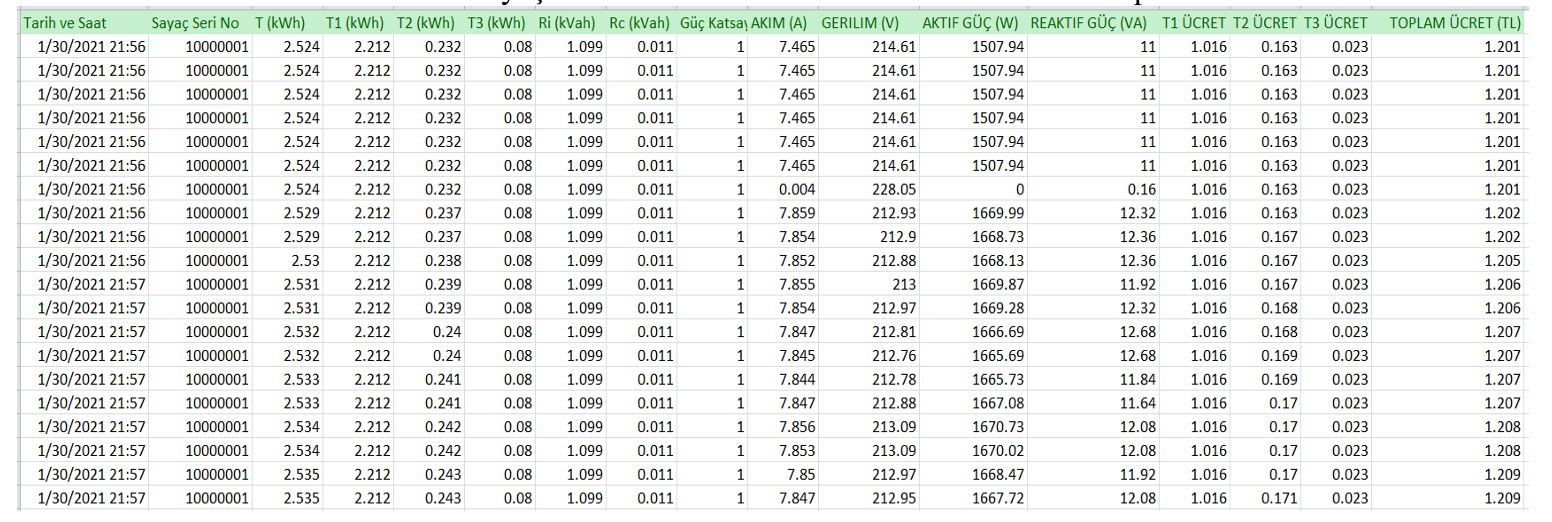
\includegraphics[width=0.8\columnwidth]{imgs/Report of Smart Meter Data in Excel Format.png}
    \caption[Short description for list of figures]{Report of Smart Meter Data in Excel Format }
    \label{fig-magnitude}
    \end{figure}%

    Another approach, "Integration of Modbus Ethernet Communication for Real-Time Electrical Power Consumption, Temperature, and Humidity Monitoring System", has been followed in order to solve the energy saving problem by using real-time data monitoring and management. In the study, electrical parameters such as voltage, current, power factor, as well as environmental variables such as temperature and humidity were collected from industrial energy analyzers. This data was recorded both locally and transferred to the cloud system via the ESP32 microcontroller. Thus, energy consumption and environmental conditions were continuously monitored, and early detection of abnormal consumption behaviors and environmental effects that would lead to loss of efficiency was provided. The measurement data obtained in the study was systematically categorized. In Table 1, data such as temperature, humidity, voltages, and currents collected from the devices used were recorded and analyzed in real time in Excel format. This data reveals the change in the temperature and humidity conditions of the electrical panel over time and the effect of this change on the energy parameters.

    \begin{figure}[H]
        \centering
        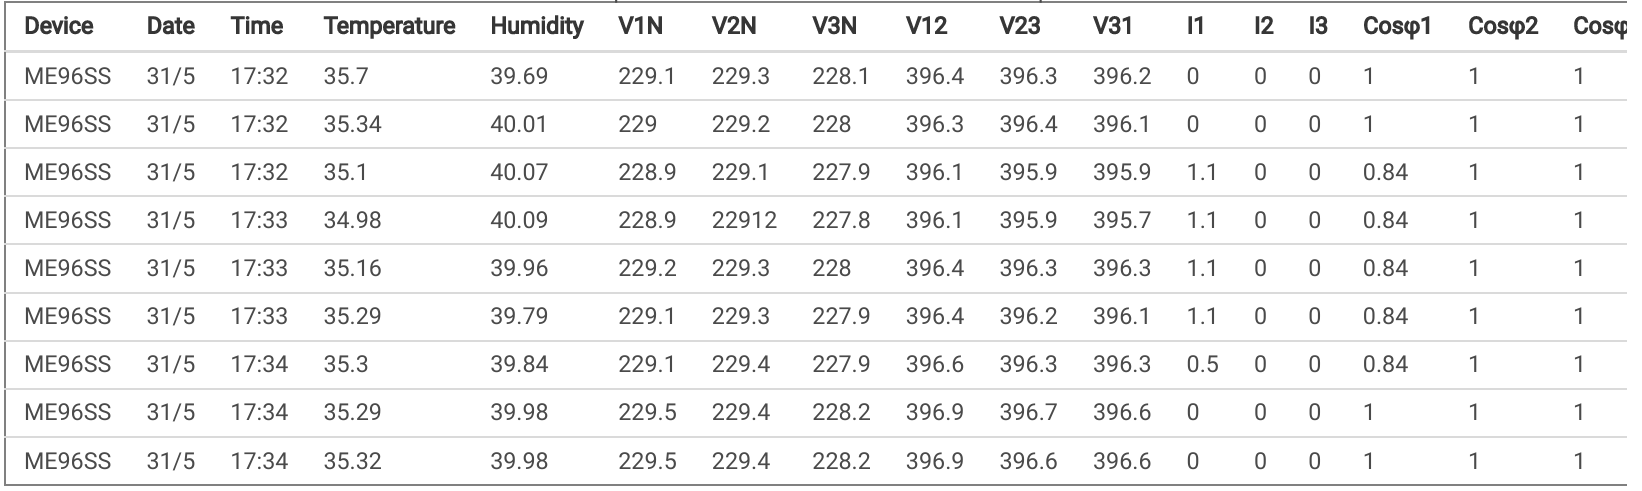
\includegraphics[width=0.8\columnwidth]{imgs/Electrical power data from the meter on the excel spreadsheet.png}
        \caption[Short description for list of figures]{Electrical power data from the meter on the excel spreadsheet }
        \label{fig-magnitude}
        \end{figure}%

        
\section{Induction Motor Energy Efficiency}

As part of a genuine literature review, the study titled “Energy Efficiency of Induction Motor Drives: State of the Art, Analysis and Recommendations” provides a detailed analysis of current approaches to improving the energy efficiency of induction motors. The authors systematically classified and analyzed 151 different literature studies in order to assess the current state of knowledge in this field.

The study emphasizes that despite global efforts to promote low-carbon energy sources, traditional fossil fuel-based systems still account for a high proportion of energy consumption. In this context, efforts to improve energy efficiency are coming to the fore. In particular, asynchronous motor drives, which are widely used in industry, account for a significant proportion of electrical energy consumption.

The study identifies five main and 48 sub-research areas aimed at improving energy efficiency and groups them under the following headings:

\begin{figure}[H]
    \centering
     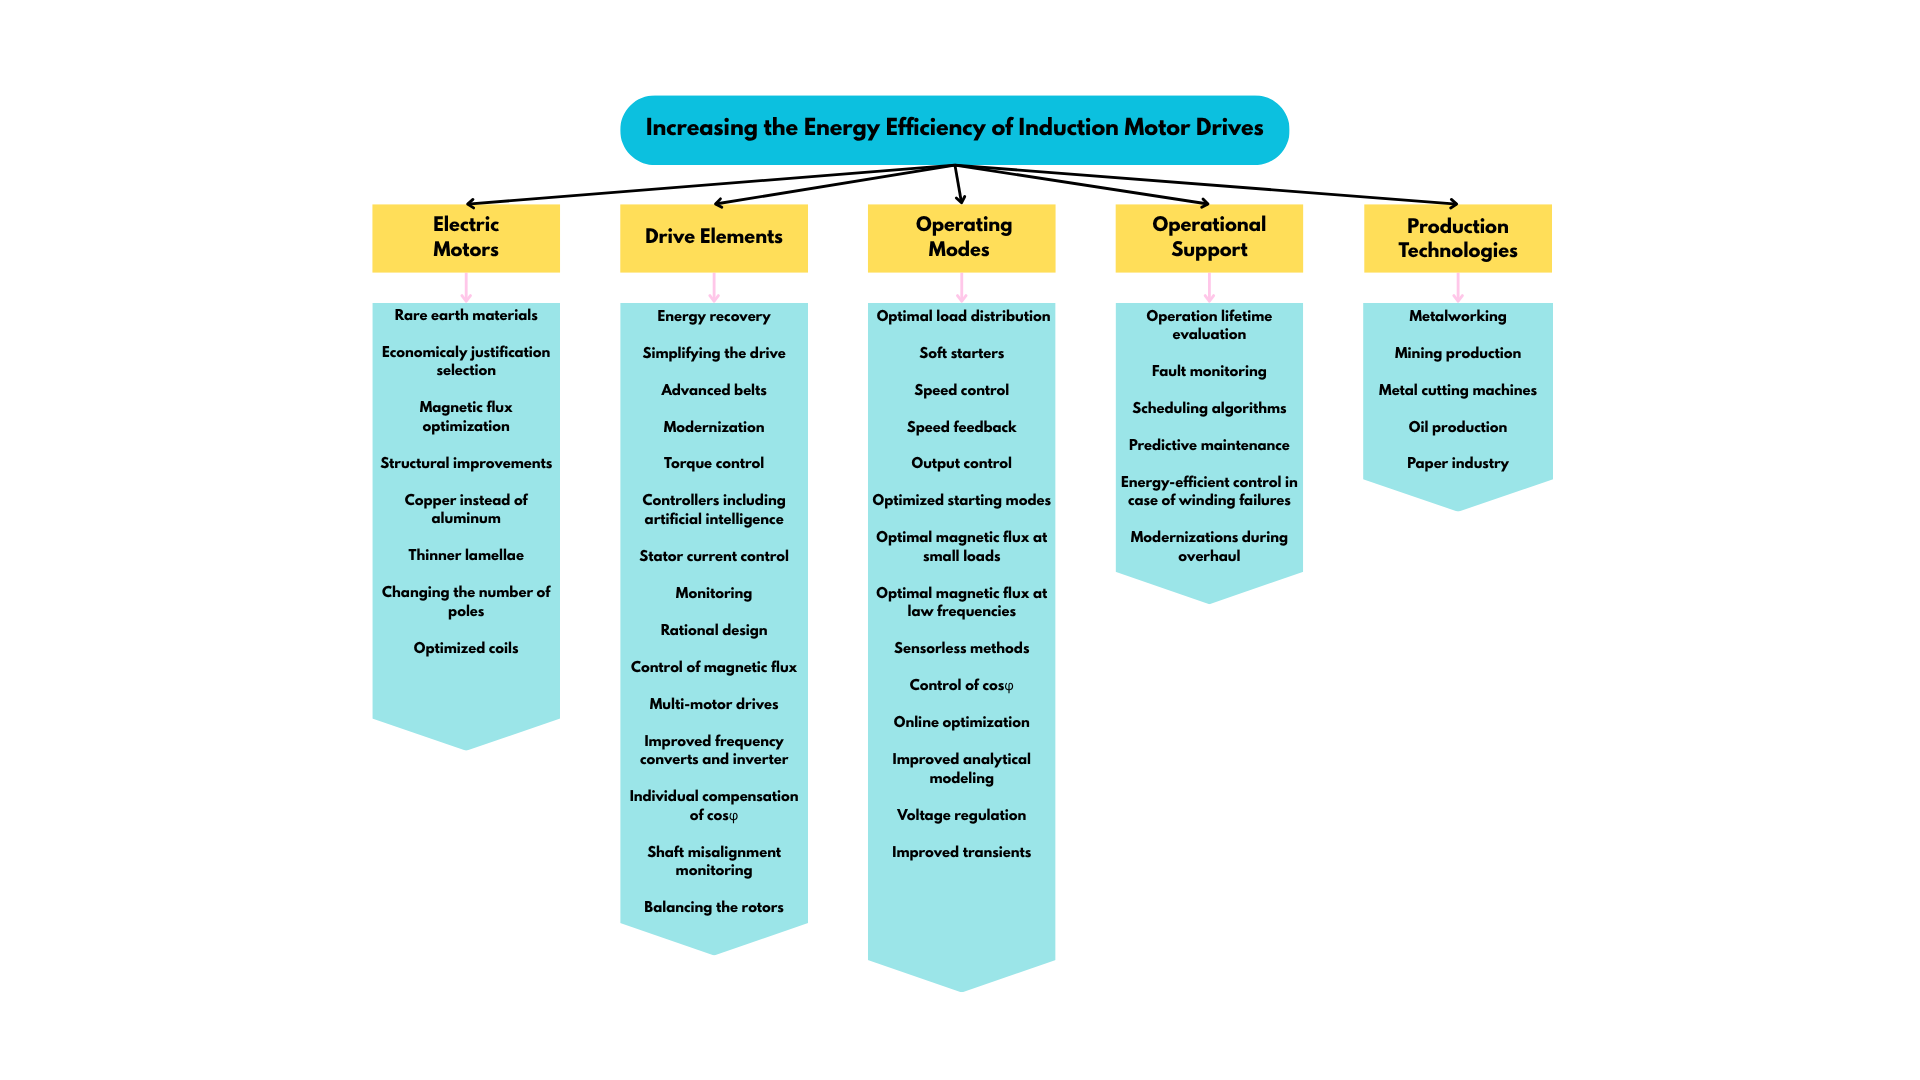
\includegraphics[width=0.8\columnwidth]{imgs/Optimal load distribution (1)} 
    \caption[Short description for list of figures]{Energy efficiency and Groups }
    \label{fig-magnitude}
    \end{figure}%

    


According to the analysis results, studies in the areas of “load distribution optimization” and “predictive maintenance” stand out in terms of the number of citations. However, it is also noted that factors such as field-based energy consumption measurements, the competencies of energy managers, and analyses of the current state of systems also play a decisive role in energy efficiency studies.

Based on the findings, it is recommended that future research prioritize issues such as the development of data collection systems, improving measurement accuracy, and creating decision support models for energy managers.

In this context, our study aims to optimize energy management through control strategies implemented on the operating mode of the asynchronous motor, thereby increasing the amount of energy saved. In line with this objective, it is planned to develop dynamic control algorithms suitable for the motor's load profile and operating conditions. This will ensure system-level efficiency and contribute to sustainability goals by reducing total energy consumption.


As part of a thorough literature review, the study titled “Endüstride Yüksek Verimli Motor Kullanımın Enerji Verimliliğine Etkileri” published by Üser et al. (2004) comprehensively examines the role of using high-efficiency motors in industry in reducing energy consumption. This study examines the energy savings and cost advantages of using high-efficiency motors instead of standard-efficiency motors in industrial facilities. The study details motor losses, efficiency calculation methods, and the technical characteristics of high-efficiency motors, and evaluates the performance of existing motors through applied measurements at Antalya ETİ Elektrometalurji A.Ş. The results indicate that transitioning to high-efficiency motors provides significant energy savings with a short payback period of approximately 19 months and offers an effective solution for improving energy efficiency in industrial facilities. The high cost of electricity compared to other energy types can provide significant cost advantages even when the savings rate is small. Electricity consumption in industrial facilities accounts for 10-25\% of total energy consumption, depending on the process, and in some cases, nearly 50\% of total energy costs are allocated to electricity. Therefore, electricity saving methods have the potential to significantly reduce total costs. Approximately 10\% of electricity consumption in industry is used for lighting and heating, while 90\% is used for electric motors. 95\% of these motors are alternating current short-circuit rotor asynchronous motors. Electric motors are used to convert electrical power into mechanical power. The fact that the majority of electrical energy in industry is consumed by motors highlights the critical importance of motor selection, operation, and maintenance in terms of energy savings.

{Losses Occurring When the Motor is Running Idle}: \\
When there is no load on the motor shaft, the rotor speed (nr) is close to the synchronous speed. The rotor speed is approximately 1\% less than the rotating field speed. In this case, the slip s is 1\%.

Asynchronous motors running at no load draw between 15\% and 50\% of their normal current (full load current) from the grid. When the motor is at no load, it draws the energy component of the current from the grid to compensate for the iron and friction losses of the stator and rotor. Additionally, it draws a certain amount of reactive component (magnetizing current). The motor's power factor at no load is low. The no-load losses can be summarized as follows: \\
• Iron losses (magnetic losses) are independent of load and remain constant.\\
• Friction (mechanical) losses are independent of load and remain constant. They may vary depending on motor speed.


Motor losses during load operation: \\
When the motor is idling, the slip amount s=1. When the load is applied, the rotor speed decreases and s increases. The cutting speed of the rotating field on the rotor windings increases. The electromotive force (emf) induced in the rotor increases. The phase currents increase. The current drawn from the grid by the motor increases. Accordingly, the losses under load can be listed as follows:\\
• Stator copper losses (primary $I^2R$ loss)\\
• Rotor copper losses (secondary $I^2R$ loss)\\
• Losses caused by load fluctuations

The energy loss rates that occur in the motors are given as percentages in Table 2.2.


\begin{table}[h!]
\centering
\begin{tabular}{|l|c|}
\hline
\textbf{Losses} & \textbf{\%} \\ \hline
Primary I\textsuperscript{2} losses & 5.6 \\ \hline
Secondary I\textsuperscript{2} losses & 2.7 \\ \hline
Core (iron) losses & 3.0 \\ \hline
Friction and windage losses & 1.4 \\ \hline
Losses due to load fluctuations & 2.3 \\ \hline
\textbf{TOTAL} & \textbf{15.0} \\ \hline
\end{tabular}
\caption{Ratios of Motor Losses}
\label{tab:losses}
\end{table}

Stator loss varies depending on stator current and resistance. The stator current expression is given in equation (2.1).

\begin{equation}
I_s = \frac{P_e}{\sqrt{3} \cdot U \cdot \cos\varphi}
\end{equation}

Here; $I_s$ is the stator current [A], $P_e$ is the electric power [W], 
$U$ is the voltage [V], and $\cos\varphi$ is the power factor. 
The rotor loss changes depending on the rotor resistance and $s$, 
and it is given in equation~(2.2).

\begin{equation}
\text{Rotor loss} = \frac{746 \cdot P_c \cdot f_w \cdot s}{1 - s}
\end{equation}


Here; $P_c$ is the output power in HP, $f_w$ is the total of friction 
and air friction losses, and $s$ is the motor slip. The rotor speed 
can never be equal to the synchronous speed of the poles $N_s$. 
In other words, the rotor speed is always less than the synchronous speed. 
There is always a slip.

Accordingly, the relationship between the speeds expressed by slip is shown in equation (2.3).

\begin{equation}
s = \frac{n_s - n_r}{n_s} \times 100
\end{equation}

The load-dependent variation of losses in an engine with up to 50 hp is shown in Figure 2.7.

\begin{figure}[H]
    \centering
    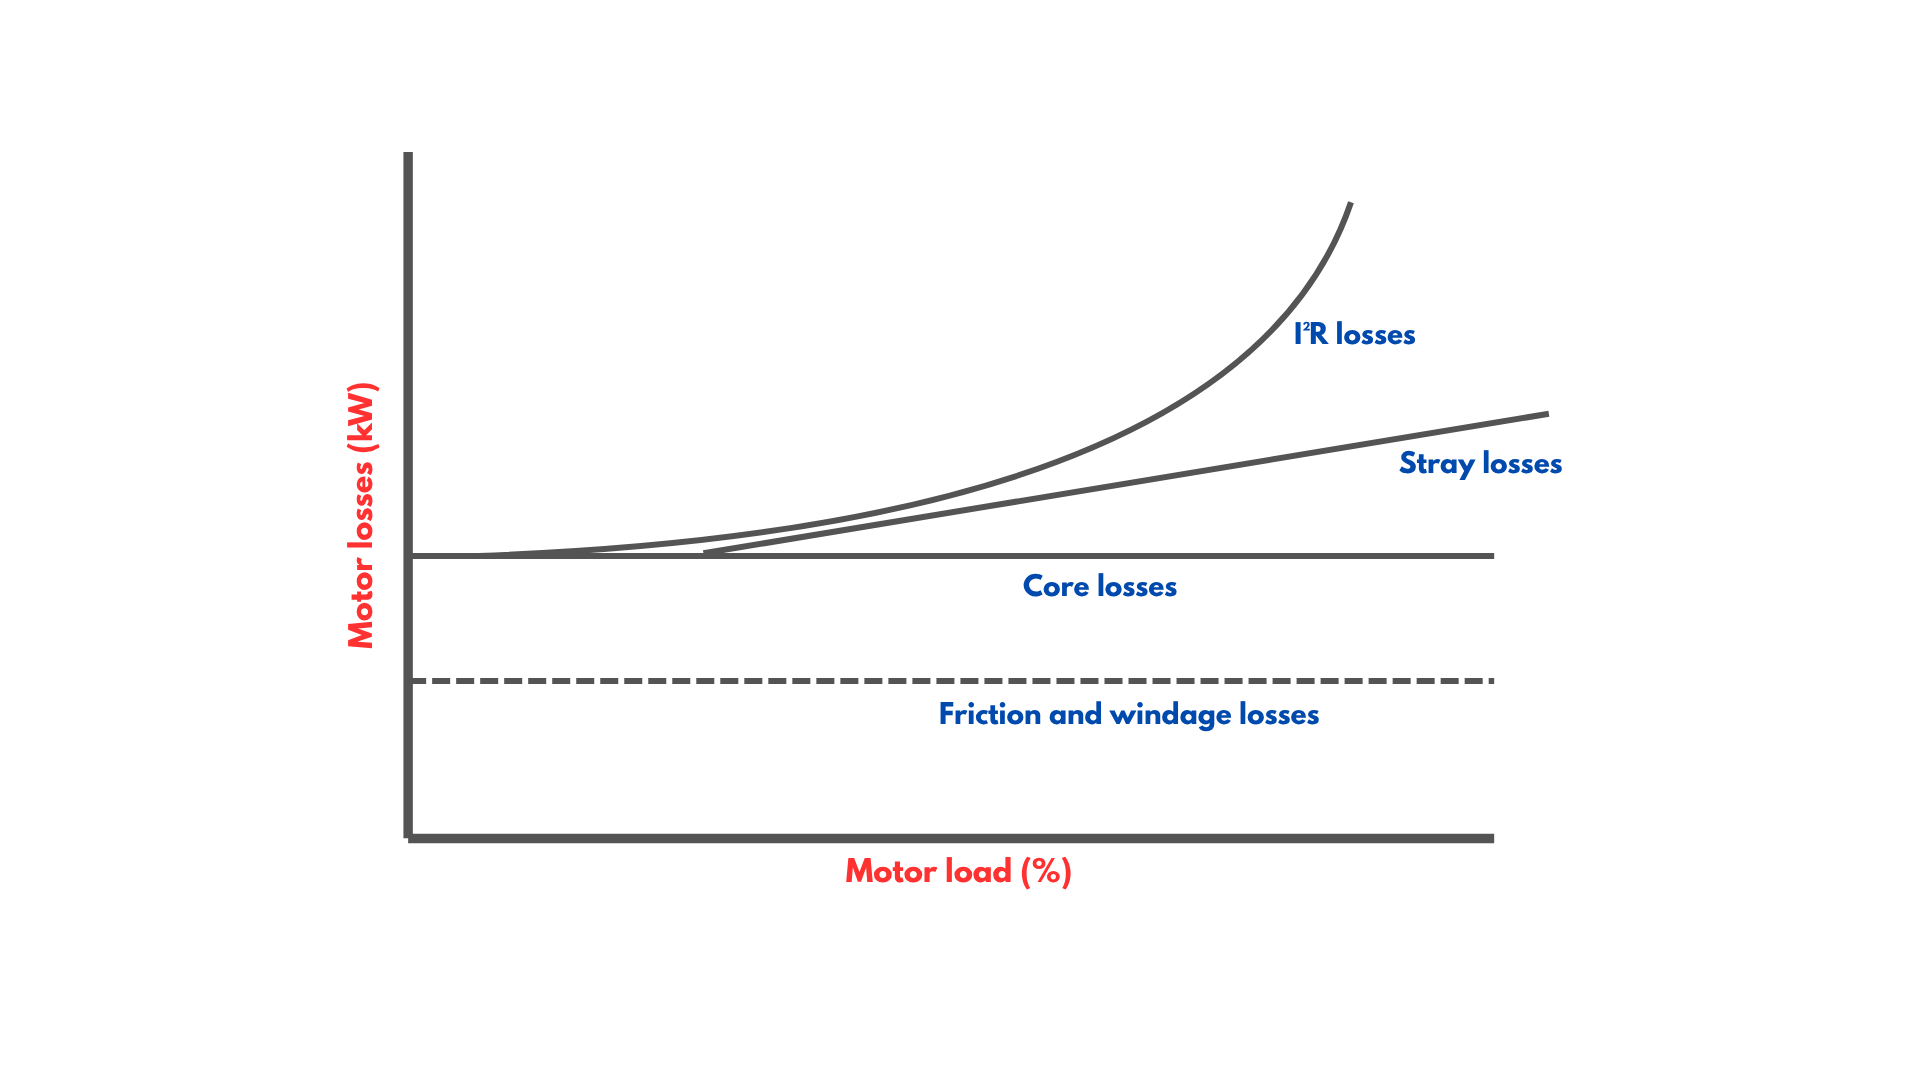
\includegraphics[width=0.8\columnwidth]{imgs/Motor losses (kW) (5).png}
    \caption[Short description for list of figures]{Changes in losses occurring in an engine up to 50 hp depending on the load }
    \label{fig-magnitude}
    \end{figure}%

In line with these theoretical foundations and experimental findings from the literature, our study focuses on applying targeted control strategies to manage the asynchronous motor’s operating modes in a way that minimizes unnecessary energy losses. By integrating real-time monitoring of motor load and slip with adaptive control algorithms, it becomes possible to dynamically adjust operating parameters to reduce copper, core, and mechanical losses. This approach not only aims to improve the overall efficiency of the motor system but also supports the long-term goals of industrial energy management by lowering operational costs and contributing to sustainability objectives.


In another study conducted by Çetin, Demir, and Çolak (2016) titled ''Energy Efficiency Analysis for Asynchronous Motors And Porsuk Vocational School Energy Efficiency Survey'', the high share of energy consumption and efficiency potential of three-phase squirrel cage asynchronous motors commonly used in industry were examined in detail. The study states that motor efficiency is the ratio of the power taken from the motor shaft to the electrical power consumed by the motor; efficiency losses are attributed to stator, rotor, iron, friction, and other losses. The information provided and the work conducted in the study are summarized as follows:

Electric motors are classified as direct current (DC) and alternating current (AC) motors. Ninety percent of electric motors used in industry are three-phase AC asynchronous motors, commonly referred to as squirrel cage motors. The reasons for this are their simple design, lower cost compared to other types, ease of maintenance, and the ability to connect directly to the AC grid. Therefore, the majority of energy is consumed by these motors. Significant energy savings can be achieved through energy efficiency studies on asynchronous motors. The use of high-efficiency electric motors is very important in reducing energy needs and costs. Efficiency in asynchronous motors is generally the ratio of the power taken from the motor shaft to the electrical power consumed by the motor. The difference between these two values represents the losses that are dissipated as heat energy and reduce motor efficiency. These losses are categorized as stator losses, rotor losses, iron losses, friction losses, and other losses. Today, these losses are being reduced, and higher energy-efficient asynchronous motors are being produced.

The first application based on efficiency in electric motors is the classification system adopted by CEMEP in 1998 to protect consumers and prevent unfair competition, known as EFF3, EFF2, and EFF1. This application covers motors ranging from 1.1 to 90 kW, with EFF3 being the lowest efficiency class and EFF1 the highest. In 2008, the International Electrotechnical Commission (IEC) published a new standard for efficiency classes, which became a European standard in 2009 and was adopted by the Turkish Standards Institute in 2010. These new efficiency classes are defined as IE1, IE2, IE3, and IE4. The IEC 60034-2-1 standard specifies the rules for motor efficiency testing methods, while the IEC 60034-30 standard explains the efficiency classes for electric motor groups directly powered by the grid. With the implementation of the IEC 60034-30-1 standard in 2014, the highest efficiency class became IE4, and the scope of efficiency was expanded. The IEC 60034-30-1 standard defines four IE (international efficiency) classes for all electric motors classified for sinusoidal voltage. According to this standard, efficiency classes are defined as shown in Table 2.3.

\begin{table}[h!]
\centering
\begin{tabular}{|l|c|}
\hline
\textbf{Standard Efficiency} & IE1 \\ \hline
\textbf{High Efficiency}   & IE2 \\ \hline
\textbf{Premium Efficiency}  & IE3 \\ \hline
\textbf{Super Premium Efficiency } & IE4 \\ \hline
\end{tabular}
\caption{Efficiency Classes}
\end{table}

The efficiency classes specified above apply to motors with a power rating between 0.75 kW and 375 kW, operating at frequencies of 50 and 60 Hz, and voltages up to 1000 V. The efficiency class of the motors is determined using the test methods specified in the IEC 60034-2-1 standard. The minimum efficiency value and the corresponding IE class of the manufactured motors must be indicated on the motor nameplates. An example of a motor nameplate is provided in Figure 2.8.

\begin{figure}[H]
    \centering
    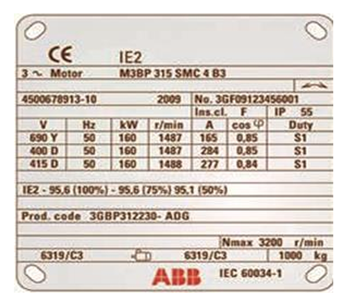
\includegraphics[width=0.6\columnwidth]{imgs/motor etiket resmi.png}
    \caption[Short description for list of figures]{Sample Motor Nameplate }
    \label{fig-magnitude}
    \end{figure}%

At the Vocational School, there are a total of 19 electric motors used for processes such as hot water transfer, irrigation, and circulation. An energy audit of these motors was carried out to find out how much energy could be saved and how long it would take for the investment cost to be recovered if the existing motors were replaced with high-efficiency motors. As a result of the inspections, the number and features of the motors used are shown in the table below.

\begin{table}[h!]
\centering
\begin{tabular}{|c|c|c|}
\hline
\textbf{Number of Engines} & \textbf{Engine Power (kW)} & \textbf{Motor Rotation Speed (rpm)} \\ \hline
11 & 0,55 & 3000 \\ \hline
5  & 1,50 & 3000 \\ \hline
2  & 1,50 & 1500 \\ \hline
1  & 0,75 & 1500 \\ \hline
\end{tabular}
\caption{Current Motor Information at School}
\end{table}

$P$ = Power ratings of the motors used (kW),\\
$\eta_1$ = Efficiency value of the old motors (\%),\\
$\eta_2$ = Efficiency value of the new motors (\%),\\
$n$ = Number of motors,\\
$t$ = Motor operating time (h),\\
$\alpha$ = Energy cost per hour (Eur/kWh)\\

Using these definitions, the calculations are performed with Equation~\ref{eq:1} and Equation~\ref{eq:2}, and the results are examined in Table~5 in the results section.

\begin{equation}
\label{eq:1}
\text{Annual Saving from Replacement} = (P \times \eta_1 - P \times \eta_2) \times \alpha \times t \times n
\end{equation}

\begin{equation}
\label{eq:2}
\text{Payback Period (Years)} = \frac{\text{Total Replacement Cost}}{\text{Annual Saving from Replacement}}
\end{equation}

In the calculations, the annual usage of the motors was assumed to be 4320 hours, and the unit cost of electricity was assumed to be 0.07 Eu/kWh. The review revealed that the motors had not been rewound previously, so the efficiency loss due to rewinding was not included in the calculation. The calculations were based on the efficiency of the motors at 100\% load (Direct Online). For motors currently in operation, the efficiency values of the motors were accepted as IE1 values defined in the IEC/EN 60034 30-1: 2014 standard. New motors were selected from the IE3 efficiency class due to the unavailability of IE4 motor production at current power levels and were included in the calculations at current purchase prices.

The issue of how to achieve efficiency and savings in asynchronous motors, which consume large amounts of electrical energy, has been addressed in conjunction with analyses of pump motors at the Vocational High School. Given the difficulties involved in generating electrical energy, it is clear that we must use it efficiently. The goal of efficient use is to reduce losses, consume less energy in production processes, provide savings to individuals or companies, and contribute to the national economy and environmental protection. Humanity's consumption of electrical energy is increasing faster than primary energy consumption, and this increase is occurring even more rapidly in our country due to our status as a developing nation. Therefore, electricity conservation should be given utmost importance, and awareness should be raised. As mentioned earlier, nearly half of total electricity consumption occurs in electric motors. Among these, pump systems account for 20\% of consumption. Therefore, implementing a high-efficiency design in pump systems would result in significant savings.

\begin{table}[h!]
\centering
\resizebox{\textwidth}{!}{%
\begin{tabular}{|c|c|c|c|c|c|c|c|c|c|c|c|}
\hline
\textbf{No} & \textbf{Process} & \textbf{Power (kW)} & \textbf{Speed (rpm)} & \textbf{Motor Qty} & \textbf{IE3 Eff.} & \textbf{Old Eff.} & \textbf{Annual Operating Hours} & \textbf{Annual Saving (EUR)} & \textbf{Motor Unit Price (EUR)} & \textbf{Total Replacement Cost (EUR)} & \textbf{Payback Period (Years)} \\ \hline
1 & Pump & 0.55 & 3000 & 11 & 0.772 & 0.658 & 4320 & 410.58 & 90 & 990 & 2.41 \\ \hline
2 & Pump & 1.50 & 3000 & 5  & 0.825 & 0.752 & 4320 & 266.87 & 130 & 650 & 2.44 \\ \hline
3 & Pump & 1.50 & 1500 & 2  & 0.853 & 0.772 & 4320 & 111.59 & 140 & 280 & 2.51 \\ \hline
4 & Pump & 0.75 & 1500 & 1  & 0.825 & 0.721 & 4320 & 39.65  & 105 & 105 & 2.65 \\ \hline
\textbf{Total} &  &  &  &  \textbf{19}&  &  &  & \textbf{828.69} &  & \textbf{2025} & \textbf{2.44} \\ \hline
\end{tabular}%
}
\caption{Porsuk Vocational School Electric Motor Analysis Results}
\end{table}

Each row of the efficiency calculation table contains the motor power and speed for the relevant process, IE1 efficiency values accepted according to IEC standards and new motor IE3 efficiency values, total operating hours of motors per year, annual savings achieved through energy savings, unit and total replacement costs of motors, and finally, the payback period of the investment. Process 1 has 11 asynchronous motors operating at 0.55 kW and 3000 rpm. The current motor efficiency values are accepted as IE1 at 65.8\%, and the recommended replacement motors are selected with an efficiency value of IE3 at 77.2\%. When calculated assuming that the motors operate for 4,320 hours annually, the efficiency improvement results in a total annual savings of 410.58 EUR for the 11 motors. The unit price of the new IE3-class motors is 90 EUR, resulting in a total investment cost of 990 EUR. When comparing the total investment cost to the annual savings, the payback period for the change is calculated to be 2.41 years.In process 2, replacing five 1.5 kW 3000 rpm motors with IE3 efficiency class motors instead of IE1 efficiency class motors results in an annual savings of 266 EUR. This recoups the total motor replacement cost of 650 EUR in 2.44 years. In Process 3, replacing two motors with a power rating of 1.5 kW and a speed of 1500 rpm results in an annual savings of 111.59 EUR. This recoups the replacement cost of 280 EUR in 2.51 years. In process number 4, the replacement of one motor with a power of 0.75 kW and a speed of 1000 rpm yields an annual savings of 39.65 EUR. As a result, the investment cost of 105 EUR is recovered in 2.65 years. In conclusion, a study conducted to improve motor efficiency classes in the system results in a total investment cost of 2025.00 EUR. As seen in the table calculations, improving motor efficiency values can result in annual energy savings of 828.69 EUR. This means that the total investment cost can be recovered in an average of 2.44 years, and significant savings can be achieved over the operational lifespan of the motors.

The connection between this study and our study is that both studies share the common goal of increasing energy efficiency. While the aforementioned research aims to achieve savings through the selection and replacement of high-efficiency motors on the hardware side, our study aims to achieve energy management through real-time monitoring of operating modes and optimization using control algorithms in existing asynchronous motors. Thus, in addition to approaches requiring hardware modernization, similar levels of efficiency gains and short payback periods can be achieved through control and monitoring-based strategies.

\section{Gaps and Limitations}

Literature reviews show that significant progress has been made in both Modbus-based energy monitoring systems and studies aimed at improving energy efficiency in asynchronous motors. However, when previous studies are examined, some common shortcomings are apparent. Firstly, Modbus-based energy monitoring applications are mostly limited to measurement, data collection, and visualization; there is insufficient focus on analyzing the collected data in real time and integrating it into motor control algorithms, i.e., transforming it into a closed-loop structure that directly provides energy optimization. This situation limits the potential energy savings capacity of the systems. On the other hand, most studies on asynchronous motor efficiency focus on hardware-based improvements (high-efficiency motor selection, motor replacement, mechanical improvements, etc.); methods for achieving energy savings without hardware changes in the existing motor fleet, using only software-based control strategies, are addressed in a limited number of cases.Furthermore, many of these studies did not take into account different load profiles, variable operating conditions, and industrial driving cycles; optimization was generally tested under constant load or laboratory conditions. Another limitation is that secondary loss components such as thermal effects, harmonic distortion (THD), and voltage imbalances are not integrated into energy management algorithms in motor efficiency analyses. In field studies focused on high-efficiency motor use, while payback periods and cost analyses are presented in detail, an integrated analysis directly comparing these scenarios with control-based software solutions is lacking. Therefore, while the existing literature provides significant knowledge on energy monitoring and motor efficiency, there is a need for comprehensive studies that combine real-time monitoring data with control algorithms, adaptively respond to different load and environmental conditions, and comprehensively compare both hardware and software-based solutions.

\section{Justification for Proposed Approach}

Modbus-based energy monitoring systems, which are widely used in industrial facilities today, ensure accurate and real-time monitoring of electrical parameters (current, voltage, power, energy consumption, etc.). However, it is not common practice to integrate this data directly into motor control algorithms to increase energy efficiency. A review of the current literature reveals that a significant portion of energy efficiency studies focus on hardware-based approaches, particularly high-efficiency motor selection and motor replacement, while the topic of achieving energy savings in existing motor fleets through software and control algorithms is addressed only to a limited extent. However, in many industrial facilities, motor replacement is not feasible in the short term due to factors such as cost, downtime, and integration challenges. At this point, real-time monitoring of the operating modes and load profiles of existing motors, combined with the application of adaptive control strategies based on the data obtained, offers significant energy savings potential without the need for hardware changes. The proposed approach aims to dynamically optimize the motor's operating mode by analyzing real-time motor data collected via Modbus RTU/TCP in terms of parameters such as load, slip, temperature, and power factor. This will reduce unnecessary copper, iron, and mechanical losses, and by operating the motor only at the required torque and speed levels, both energy consumption will be reduced and equipment lifespan will be extended. This method, as a low-cost software-based solution, can provide similar efficiency increases to methods requiring hardware modernization, offer industrial-scale applicability with short payback periods, and contribute to sustainability in the field of energy management.  


\clearpage